\chapter{Node-level performance modeling of sparse triangular solve}
\label{c:modeling}

Even in scientific computing, simulation code development often lacks a basic understanding of performance bottlenecks and relevant optimization opportunities. In this chapter we will use a structured model-based performance engineering approach on the compute node level for a fundamental kernel operation in sparse factorization solvers. We aim at a deep understanding of how code performance comes about and which hardware bottlenecks might apply. The pivotal ingredient of this process is a performance model which links software requirements with hardware capabilities. Such models are often simplified such as the well-known Berkeley roofline model or the Erlangen ECM model, but it leads to deeper insights and strikingly more accurate runtime predictions.

The package PARDISO\footnote{A discussion of the algorithms used in
PARDISO, the user manual, and more information on the solver can be found at
\url{http://www.pardiso-project.org}}
is a thread-safe, high-performance, and memory-effi\-cient,
serial and parallel solver for the direct solution of unsymmetric
and symmetric sparse linear systems on shared memory multiprocessors.
The solver uses a combination
of left- and right-looking Level-3 BLAS supernode techniques
(\cite{AndBBDDDGHMOS99}).
In order to improve sequential and parallel sparse
numerical factorization performance, the algorithms are based on
a Level-3 BLAS update and pipelining parallelism is exploited with
a combination of left- and right-looking supernode techniques.

PARDISO calculates the solution of a set of sparse linear equations
with multiple right-hand sides, using a parallel $LU$, $LDL^T$, or $LL^T$
factorization. PARDISO supports a wide range of sparse matrix types and
computes the solution of real or complex,
symmetric, structurally symmetric or unsymmetric, positive definite,
indefinite or Hermitian sparse linear system of equations on shared-memory
multiprocessing architectures.

The parallel pivoting methods for unsymmetric matrices allow complete supernode pivoting in order to ensure numerical stability and scalability during the factorization process. For sufficiently large problem sizes numerical experiments demonstrate that the scalability of the parallel algorithm is nearly independent of the shared-memory multiprocessing architecture and a speedup of up to seven using eight processors has been observed. The package is implemented using multithreading using OpenMP directives. PARDISO performs the analysis steps depending on the structure
of the input matrix $A$. See \cite{Bollhofer2020} for further details.

For comparison and to motivate the usage of the PARDISO solver, we run initial benchmarks on varouos matrices. Here we used CHOLMOD~(\cite{cholmod2008,doi:10.1137/1.9780898718881}), MUMPS~(\cite{amestoy-2000,amestoy-2001,amestoy-2006}), and PARDISO~(\cite{schenk-2004,kuzmin-2013}) solvers. For CHOLMOD and MUMPS we set METIS reordering, so all solvers have about the same factors. We measured duration of the forward/backward substitution for our benchmark
matrices. The results for the Ivy Bridge system are shown in Figure~\ref{fig:solvers}.

%
\begin{figure}[tp]
  \centering
	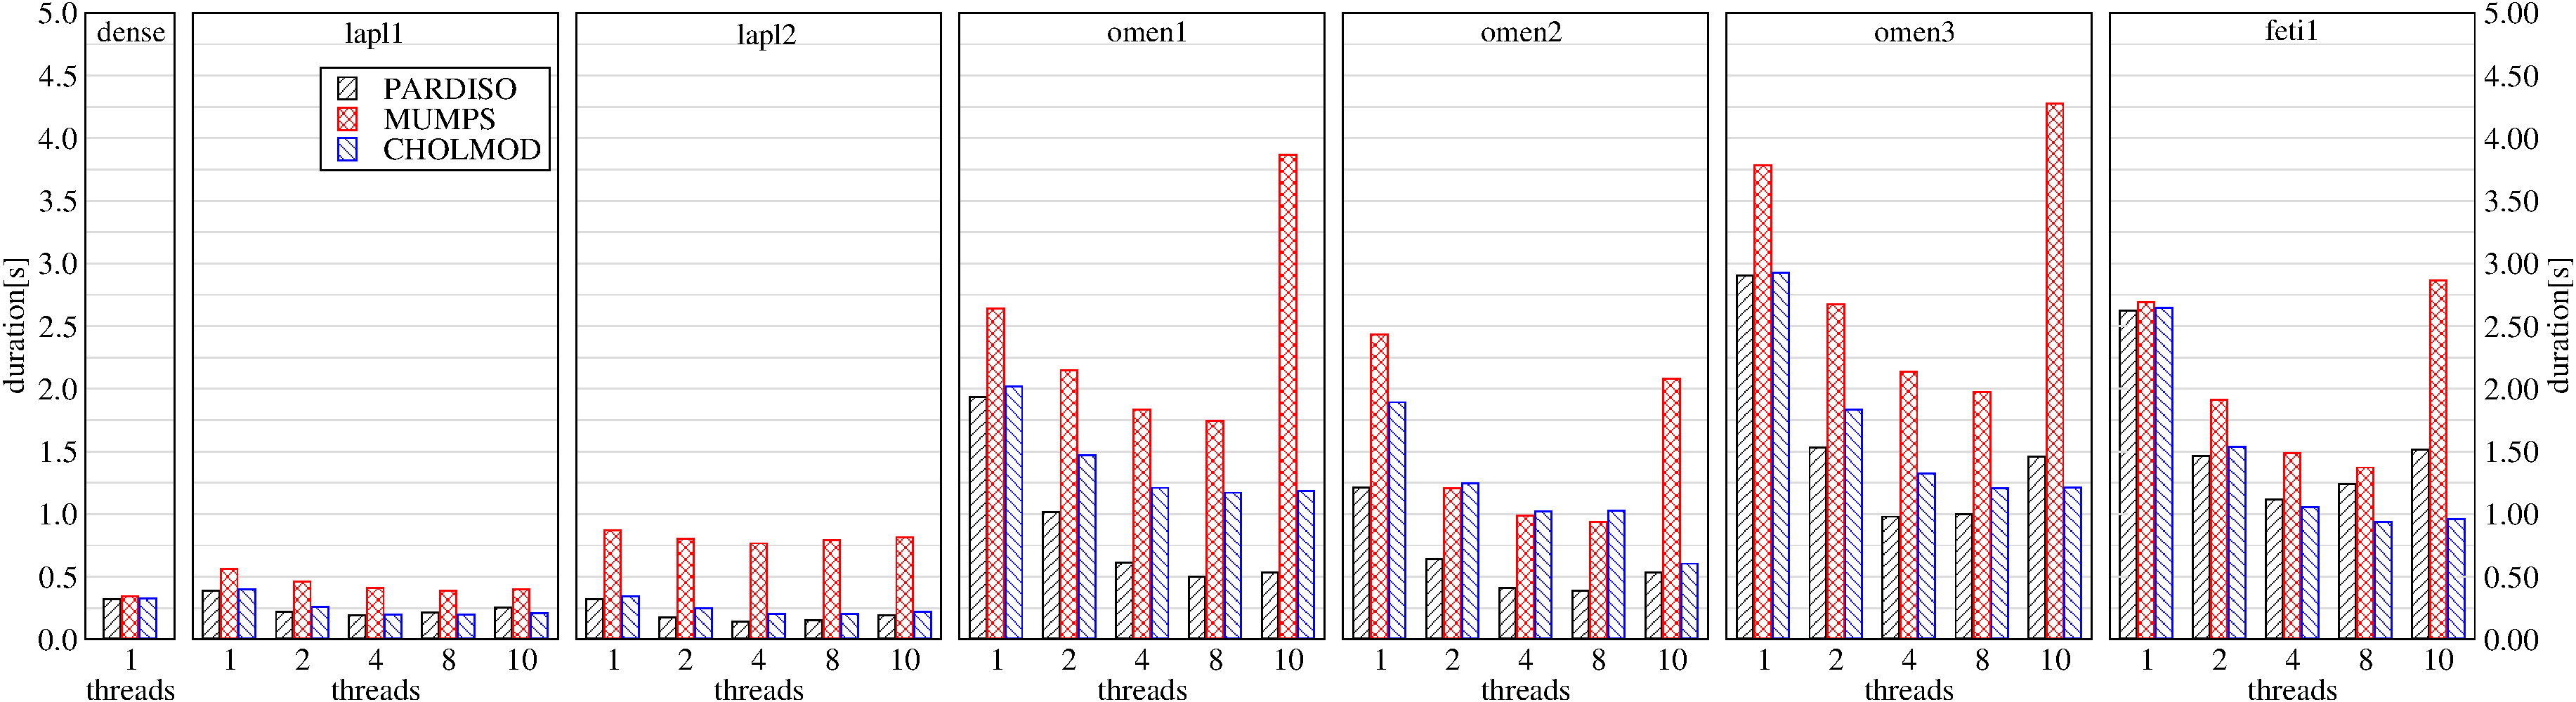
\includegraphics[width=\textwidth,clip=true]{images/SolverComparison}
   \caption{Duration of forward/backward substitution for the dense, lapl1, and lapl2 matrices for different sparse direct solvers on the IVB system.}
  \label{fig:solvers}
\end{figure}

In this chapter, we will mainly analyze the data transfer between the different cache levels and the FLOPs performed during the sparse triangular solve phase. The results of this analysis are used as input for our performance model. Therefore, we mostly inspect the different instantiations of the loops resulting from Algorithms~\ref{alg:algo:fw} and \ref{alg:algo:bw} on page \pageref{alg:algo:fw} and \pageref{alg:algo:bw}. We only consider the innermost loops because all the arithmetics are performed here. Our assumption is that the instructions regarding control variables of the loops are negligible, hence we do not them into account.
%Here, we only consider the innermost loops and do not
%distinguish between updates of~\vr{} or temporary arrays~\vtemp{}.

\section{Algorithm and data structures of sparse triangular solve}
% \section{Algorithm and Data Structures of the Forward/Backward Substitution}

\label{sec:algo}

Let $A$ be an $N \times N$ matrix and $x$ and $b$ be vectors of size $N$.
The linear system $A x = b$ is solved via $LDL^T$ decomposition by factorizing $A$
into a lower diagonal matrix $L$ and a diagonal matrix $D$ 
such
that $A =
LDL^T$.
The system is then solved in three steps. First,
$
  \label{eq:fw}
  Ly=b
$
is solved via forward substitution. This is followed by a diagonal solve
$
  \label{eq:dg}
  Dz=y
$
and, afterwards, the resulting $z$ vector is used to solve for the solution vector
%
$
  \label{eq:bw}
  L^Tx=z
$
% 
% via backward substitution. In sparse solver packages, such as, e.g.,
% PARDISO~\cite{schenk-2004}, 
via backward substitution. In 
PARDISO, 
the forward substitution is performed columnwise, starting with the
first column.
%mw first column, as depicted in Fig.~\ref{algo:triangular}~(a).
The data dependencies here allow us to store vectors $y$, $z$, $b$, and $x$ in
only one vector $r$. 

%\begin{figure}[t]
%  \centering
%    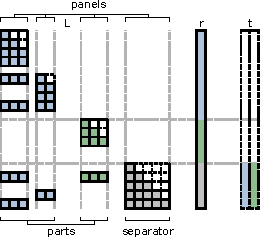
\includegraphics[width=0.55\linewidth,clip=true]{images/parts-panels-separator}
%  \caption{Sparse matrix data structures in PARDISO. Adjacent columns of $L$ exhibiting the same
%structure form panels also known as supernodes.
%Groups of panels which touch independent elements of the right-hand side $r$ are
%parts. The last part in the lower triangular matrix $L$ is called the separator.}
%  \label{fig:algo:ds}
%\end{figure}

The sparse matrix is stored in a PARDISO specific format shown in
Figure~\ref{fig:algo:ds}.
Adjacent columns exhibiting the same row sparsity structure form a
\textit{panel}, also known as a \textit{supernode}.
A panel's column count is called the \textit{panel size} $\panelsize$.
The columns of a panel are stored consecutively in memory excluding the zero
entries. 
Note that columns of panels are padded in the front with zeros so they get the 
same length as the first column inside their panel. 
The padding is of utmost importance for the PARDISO solver to use Level-2/3
BLAS and LAPACK functionalities. Please see~\cite{Bollhofer2020} for more
details.
Furthermore, panels are stored consecutively in the array \vlnz{}.
Row and column information is now stored in accompanying arrays.
%2 The \texttt{xsuper} array stores for each panel the index of its first column. 
%Also note that here column indices are the running count of nonzero columns.
Column indices are used as indices into the array \vxlnz{} to look up the
start of
the column in the array \vlnz{} which contains the numerical values of the factor $L$.
%2Panel~$p$ starts then in \vlnz{} at \vxlnz\texttt{[xsuper[p]]}.
To determine the row index of a column's element array \vindx{} is
used, which holds the row indices for each panel.
%2 The start of a panel inside \vindx{} is found via \vxindx{} array.
%2 The first row index of panel~$p$ is \vindx\texttt{[\vxindx[p]]}.

%2 For serial execution this information is enough. 
%2 However, during parallel forward/backward substitution concurrent updates to
%2 the same entry of \vr{} must be avoided.
For parallel execution concurrent updates to the same entry of \vr{} must be
avoided.
The \textit{parts} structure contains the start (and end) indices of the panels
which can be updated independently as they do not touch the same entries of $r$.
Two parts, colored blue and green, are shown in Figure~\ref{fig:algo:ds}.
The last part in the bottom right corner of $L$ is special and is called the 
\textit{separator} and is colored gray.
%
Parts which would touch entries of \vr{} in the range of the separator perform 
their updates into separate temporary arrays \vtemp{}.
Before the separator is then serially updated, the results of the temporary
arrays are gathered back into \vr{}. 
The backward substitution works the same, just reversed, and
updates to different temporary arrays are not required.
Figure \ref{fig:ecm-parallel-model} shows a possible execution of forward solve. The nested dissection reordering assigns to every partition about the same number of columns. However, panels in different partitions can have different size (number of columns). Then different threads execute differently unrolled code, as can be seen on the left side of Figure \ref{fig:ecm-parallel-model}. For easier modeling we assume the execution of the unrollings is sorted and evenly distributed over cores, as shows the right side of Figure \ref{fig:ecm-parallel-model}.

\begin{figure}[t]
  \centering
  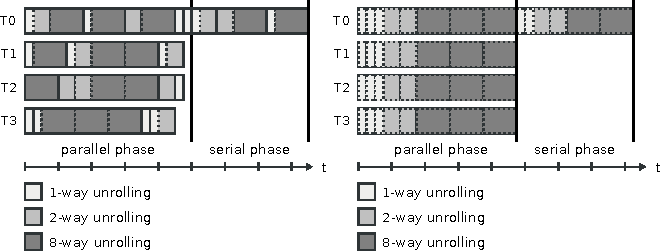
\includegraphics[width=0.9\textwidth,clip=true]{images/ecm-parallel-model}
   \caption{Possible real execution of forward solve. In the parallel phase cores can execute differently unrolled loops at the same time. For easier modeling the execution of the unrollings is sorted and evenly distributed over all cores.}
  \label{fig:ecm-parallel-model}%
\end{figure}

%\begin{algorithm}[t]
%  \begin{algorithmic}[1]
%    \Procedure{Sparse Forward Substitution}{}
%      \For{part in parts} \Comment{parallel execution}
%        \For{panel p in part}
%          \For{\textcolor{blue}{column $j$ in panel p}} \Comment{unroll} \label{alg:fw:1}
%            \State i = \nxindx{}[p] + offset
%
%            \For{k = \nxlnz[j] + offset; k < sep; ++k}\label{algo:fw:rloop}
%                \State row = \nindx[i++]
%                \State \nr[row] - =  \nr[j] \nlnz[k] \Comment{indexed DAXPY}
%            \EndFor\label{algo:fw:rloop:end}
%            \For{k = sep + 1; k < \nxlnz[j+1]; ++k}\label{algo:fw:seploop}
%                \State row = \nindx[i++]
%                \State \ntemp[row,p] -=  \nr[j] \nlnz[k] \Comment{indexed DAXPY}
%            \EndFor\label{algo:fw:seploop:end}
%          \EndFor
%        \EndFor
%      \EndFor
%
%      \State
%      \State r[i] = r[i] - sum(\ntemp[i,:])  \Comment{gather temporary arrays}
%      \State
%
%      \For{panel p in separator} \Comment{serial execution}
%        \For{\textcolor{blue}{column $j$ in panel p}} \Comment{unroll}\label{alg:fw:2}
%            \State i = \nxindx[p] + offset
%
%            \For{k = \nxlnz[j] + offset; k < \nxlnz[j+1]; ++k}\label{alg:fw:3}
%                \State row = \nindx[i++]
%                \State \nr[row] -=  \nr[j] \nlnz[k] \Comment{indexed DAXPY}
%            \EndFor
%        \EndFor
%      \EndFor
%    \EndProcedure
%  \end{algorithmic}
%  \caption{Forward substitution in PARDISO. Note that in the case of serial
%execution, separated updates to temporary arrays in lines
%\ref{algo:fw:seploop}--\ref{algo:fw:seploop:end} are not necessary
%and can be handled via the loop in lines
%\ref{algo:fw:rloop}--\ref{algo:fw:rloop:end}.}
%  \label{alg:algo:fw}
%\end{algorithm}
%
%\begin{algorithm}[tp]
%   \begin{algorithmic}[1]
%     \Procedure{Sparse Backward Substitution}{}
%       \For{panel $p$ in sep. rev.} \Comment{serial execution}
%         \For{\textcolor{blue}{col. $j$ in panel $p$ rev.}} \Comment{unroll}\label{alg:bw:1}
%            \State i = \nxindx[p] + offset
%
%            \For{k = \nxlnz[j] + offset; k < \nxlnz[j+1]; ++k}\label{alg:bw:3}
%                \State row = \nindx[i++]
%                \State \nr[j] -= \nr[row] \nlnz[k] \Comment{indexed DAXPY}
%            \EndFor
%
%            \State offset = offset - 1
%          \EndFor
%        \EndFor
%
%        \State
%
%        \For{part in parts} \Comment{parallel execution}
%          \For{panel $p$ in part rev.}
%            \For{\textcolor{blue}{col. $j$ in panel $p$ rev.}} \Comment{unroll}\label{alg:bw:2}
%
%              \State i = \nxindx[p] + offset
%
%              \For{k = \nxlnz[j] + offset; k < \nxlnz[j+1]; ++k}
%                \State row = \nindx[i++]
%                \State \nr[j] -=  \nr[row] \nlnz[k] \Comment{indexed DAXPY}
%              \EndFor
%
%              \State offset = offset - 1
%
%            \EndFor
%          \EndFor
%        \EndFor
%        \EndProcedure
%   \end{algorithmic}
%   \caption{Backward substitution in PARDISO. Separator (sep.), parts, and
%panels are iterated over in reversed (rev.) order.}
%   \label{alg:algo:bw}
%\end{algorithm}


% The complete forward backward substitution is listed in
% algorithm~\ref{alg:algo:fw} and~\ref{alg:algo:bw}, respectively.
% If no parallel execution is required then panels are updated successively in
% serial and during forward substitution updates to temporary arrays are not
% necessary.
The complete forward substitution is listed in Algorithm~\ref{alg:algo:fw}.
If no parallel execution is required then panels are updated successively in
serial, and during forward substitution, updates to temporary arrays are not
necessary.
Please note that through the dense storage of panels, indirect accesses to \vr{}
are required, resulting in an ``indexed DAXPY''-like operation, which prohibits a
straightforward vectorization.
% For performance reasons (discussed later in section~\ref{sec:pam}) the loops over the
% columns (blue text) in algorithms~\ref{alg:algo:fw} and~\ref{alg:algo:bw} are $1$-, $2$-,
% and $8$-way unrolled.
For performance reasons (discussed in Section~\ref{sec:pm:dt:wu}) the
loops over the columns (blue text) in Algorithm~\ref{alg:algo:fw} are $1$-,
$2$-, and $8$-way unrolled.
%\mycomment{OR: Blau wird im Druck nicht gut sichtbar sein. Ist uns das egal,
%weil wir sowieso nur vom PDF ausgehen? MW: ja davon wuerde ich ausgehen.}
The algorithm for the backward substitution in Algorithm~\ref{alg:algo:bw} 
looks nearly the same, except that
the serial part is executed first, which is then followed by the parallel section.
%

Parallel handling of the separator during the forward and backward
substitution is in principle possible.
Hereby the loops over the rows in line~\ref{alg:fw:3} of Algorithm~\ref{alg:algo:fw}
and line~\ref{alg:bw:3} of Algorithm~\ref{alg:algo:bw} would be parallelized.
However, typically the number of rows for sparse problems is too small to
benefit from this optimization and at worst it could introduce significant
overhead.

\section{Performance analysis of sparse triangular solve}
%\section{Analysis of the Forward/Backward Substitution} 
\label{sec:sds}

% \mycomment{OR: Werden die Daten analysiert oder ihr Transfer? MW: der Transfer
% natürlich :)}
%In this section, we analyze the data transfer between the different cache levels
%and the FLOPs performed during  the
%sparse triangular solve phase.
%%\sout{\OR the forward/backward substitution.}
%% \mycomment{OR: Fehlender Bezug durch ``which''. MW: OK}
%The results are used as input for our performance model
%to be
%established in the next section.
%%
%Therefore, we inspect the different instantiations of the loops resulting from
%Algorithm~\ref{alg:algo:fw} and~\ref{alg:algo:bw}.
%% \mycomment{``Hereby'' heisst ``hierdurch'', nicht ``hierbei''}
%Here, we only consider the innermost loops and do not
%distinguish between updates of~\vr{} or temporary arrays~\vtemp{}.

All entries %\sout{coefficients} 
of the matrix $L$
% \mycomment{OR: Bezeichnung ``coefficients'' hier gut? MW: entries? OR: OK.}
are stored as double-precision floating point
numbers in the vector \vlnz{}, consuming $8$\,B (byte) each.
Elements of the vector \vxlnz{} (column start indices in the vector \vlnz{}) and vector \vxindx{} (start
indices of row indices for each panel) are stored as $8$\,B integers,
whereas for the entries of the vector \vindx{} (row indices for each panel) $4$\,B integers
are used.
\enlargethispage*{\baselineskip}

\subsection{Data transfers and FLOPs without unrolling}
\label{sec:pm:dt}
\label{sec:pm:dt:wou}

% \begin{figure}[t]
%   \centering
%  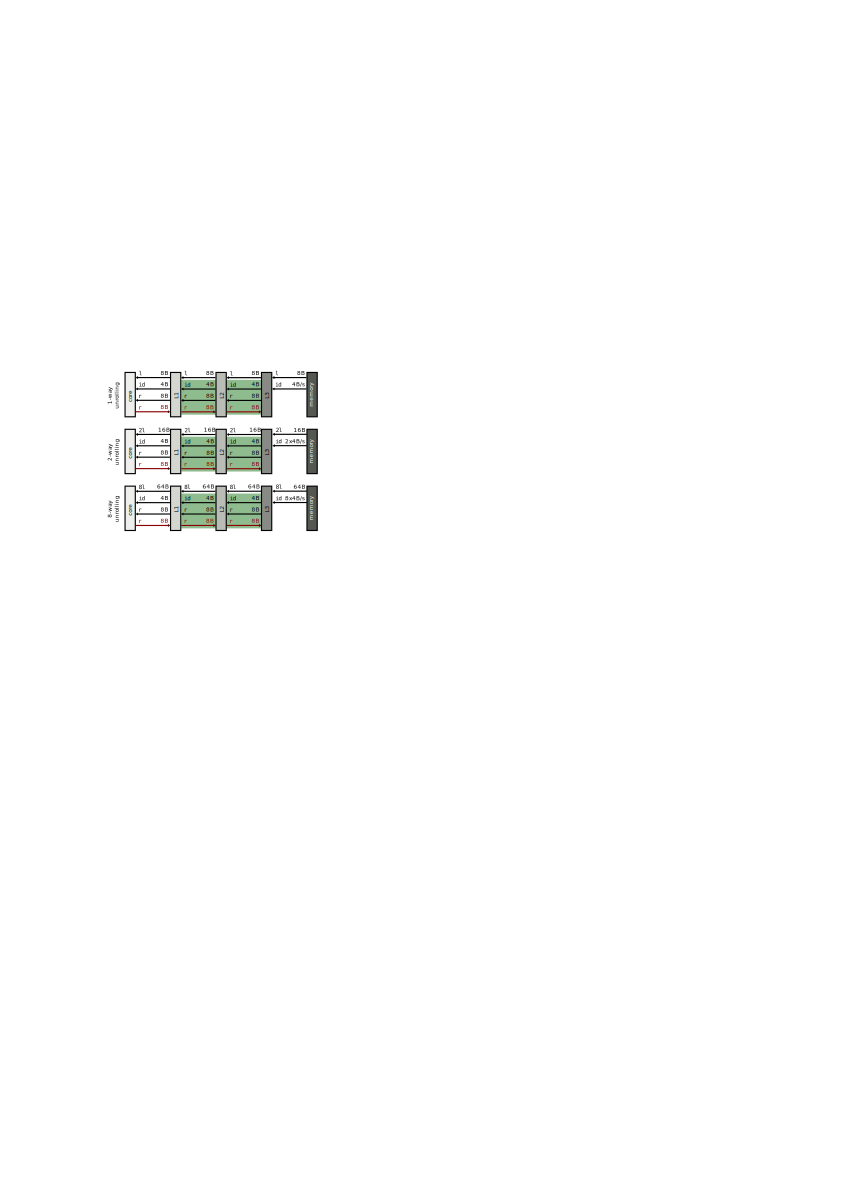
\includegraphics[width=0.43\textwidth,clip=true]{images/ecm-datatransfers}
%   \caption{Data transfers for one iteration of the forward
%     (including red text and arrows) and backward (without red text and arrows)
%     substitution when $1$-, $2$-, or $8$-way column unrolling is applied.
%     Thereby $1$, $2$, or $8$ nonzero elements of \vlnz{} are processed,
%     respectively.
% %    Loading of \vindx{} from memory (blue boxes) is only included in the model 
% %    if the panel size $s \le 8$.
% % From which cache level \vr{} is reused (green boxes) depends on the size of the
% % active part. If the active part is large it must be reloaded from
% % L3 cache. With decreasing size it can fit into L2 or even L1 cache.
% % This holds also true for \vindx{}, but additionally depends on the panel size.
%   }
%   \label{fig:ecm:data}
% \end{figure}
% 

In the most simple case no unrolling is applied and the innermost loop of
forward substitution from Algorithm~\ref{alg:algo:fw} looks like
% \mycomment{OR: sollte der Alg.~\ref{alg:algo:fw} nicht
% eine Float-Umgebung bekommen? MW: algorithm ist doch eine float-Umgebung.
% OR: Habe mich vertan.
% }
%
\begin{algorithmic}[1]
  \setcounter{ALG@line}{20}
  \For{k = \nxlnz[j] + offset; k < \nxlnz[j+1]; ++k}
      \State row = \nindx[i++]
      \State \nr[row] -= \nr[j] \nlnz[k]
  \EndFor
\end{algorithmic}%
%\vspace{-\baselineskip}
\noindent%
%
As the loops from lines $6$--$9$ and $10$--$13$ are in principle identical to
the loops in lines $21$--$24$, we only discuss the latter.
%
During each iteration one nonzero is processed, two FLOPs are performed,
namely, a multiplication and an addition, and the following elements get
loaded and stored: loaded: \vindx{} ($4$~\,B), \vr{} ($8$~\,B), \vlnz{}
($8$~\,B); stored: \vr{} ($8$~\,B).

How much data are transferred inside the cache hierarchy depends on the size of
the caches, their replacement strategies, the size of \vr{}, the average panel
size, as well as the structure of the panels, i.e.,\ which part of \vr{} is
accessed.
Here we assume \vr{} is small enough to be kept at least in last level cache
(LLC) and temporal locality ensures it is not evicted.
%
Row indices in \vindx{} for a panel are loaded from memory for the panel's first
column and then are reused during each iteration over the panel's remaining
columns from the LLC in the worst case.
With panel size $\panelsize=1$, for each element of \vlnz{} one row index is
transferred and no reuse is possible.
In general reuse is only possible, starting with a panel's second column for
panel sizes $\panelsize \ge 2$.
%
Coefficients of \vlnz{} are always streamed in from memory, as they are
used only once and the array \vlnz{} is typically too large to be kept in LLC.
Figure~\ref{fig:ecm:data-fw} visualizes the transfers assuming three cache levels
and \vr{} is cached in LLC.
While iterating over panels and columns, the number of column elements
decreases as $L$ is a lower triangular matrix.
Thereby the number of used elements from \vr{} also decreases, which we call the
active part of \vr{}.
At some point the active part can be completely kept in the L2 or even the L1 cache.
This also holds true for \vindx{}, except when a new panel starts, then
the panel's row indices must first be loaded from memory.
With Intel L2 cache 256\,kB and L1 cache 32\,kB, a maximum of about 13000 and 1600 elements of \vr{}, \vindx{}, and \vlnz{} could fit into the L2 and L1 caches, respectively. However, due to the associativity and replacement strategy of the cache and the need to store other data, it is reasonable to expect only half of the size can be used. We can expect if the active part of \vr{} is less than about 6000 elements, it can be kept in the L2 cache, and if it is less than about 800 elements it fits into the L1 cache.
\clearpage

\begin{figure}[t]
  \centering%
%  \includegraphics[width=0.3\textwidth,clip=true]{images/ecm-datatransfers-1}
%  \includegraphics[width=0.3\textwidth,clip=true]{images/ecm-datatransfers-2}
%  \includegraphics[width=0.3\textwidth,clip=true]{images/ecm-datatransfers-8}
  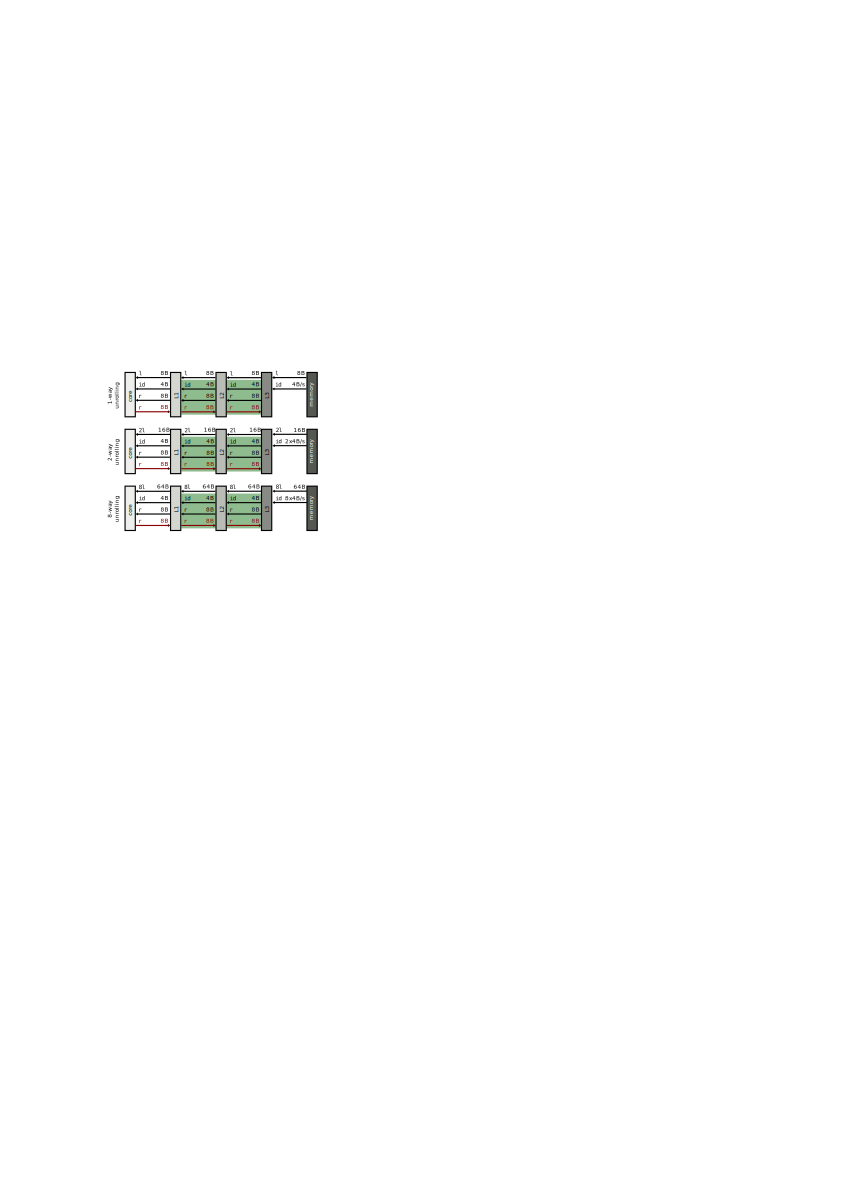
\includegraphics[width=0.75\linewidth,clip=true]{images/ecm-datatransfers-fw}
  \caption{Data transfers for one iteration of the forward
    substitution when \protect\linebreak $1$-, $2$-, or $8$-way column unrolling is applied
    for a panel with panel size $s$.
    Thereby $1$, $2$, or $8$ nonzero elements of \vlnz{} are processed,
    respectively.
%    Loading of \vindx{} from memory (blue boxes) is only included in the model
%    if the panel size $s \le 8$.
% From which cache level \vr{} is reused (green boxes) depends on the size of the
% active part. If the active part is large it must be reloaded from
% L3 cache. With decreasing size it can fit into L2 or even L1 cache.
% This holds also true for \vindx{}, but additionally depends on the panel size.
  }
  \label{fig:ecm:data-fw}
\end{figure}

%
%1 The active part of \vr{} can be kept inside a certain cache size $c_s$, when
%1 concurrently also one column of \vlnz{} and the active part of \vindx{} fit into
%1 this cache level.
%1 Let $n_j$ the length of column $j$. 
%1 If $L$ is dense, like for the dense matrix, then if $n_j \le c_s/(8\,\text{B} + 8\,\text{B} +
%1 4\,\text{B})$ holds true all active parts fit into the cache.
%1 %
%1 If instead in the worst case $L$ is sparse so that only one element out of a cache
%1 line from \vr{} is accessed
%1 then $n_j \le c_s/(8\,\text{B} + 64\,\text{B} + 4\,\text{B})$ is required.
%1 %
%1 Note that already when the active part of \vr{} slightly exceeds the determined
%1 limits already partial caching in the same cache level takes place\footnote{If
%1 we
%1 load a vector which exceeds the cache size several times it must be completely
%1 reloaded during each iteration. 
%1 However, if the cache utilizes a least recently used policy and the vector's
%1 size is in the range of the cache size $c_s$ and $c_s + w_s$, where $w_s$
%1 denotes the way size of the cache, then still parts of the vector are held in
%1 the cache and need not to be reloaded.
%1 The way size of a cache is defined as the product of the cache's number of sets
%1 and the cache line size.}.

The innermost loop of the backward substitution from
Algorithm~\ref{alg:algo:bw} is %looks like
% The innermost loop from lines $5$--$9$ is the same as the one from lines
% $17$--$20$ of the backward
% substitution from Algorithm~\ref{alg:algo:bw}, which we only discuss the former,
% which looks like 
%
\begin{algorithmic}[1]
\setcounter{ALG@line}{4}
  \For{k = \nxlnz[j] + offset; k < \nxlnz[j+1]; ++k}
    \State row = \nindx[i++]
    \State \nr[j] = \nr[j] - \nr[row] \nlnz[k]
  \EndFor
\end{algorithmic}%
%\vspace{-\baselineskip}
\noindent%
%
As this loop from lines $5$--$8$ is the same as the one from lines $16$--$19$,
all following statements hold true for both. 
%
As with forward substitution one nonzero is processed, two FLOPs are performed,
but only loads occur: \vindx{} ($4$~\,B), \vr{} ($8$~\,B), and \vlnz{} ($8$~\,B).
Note that $j$ is unchanged in the innermost loop, hence $\nr[j]$ always refers
to the same element and is not considered for the data transfer analysis.
%
Figure~\ref{fig:ecm:data-bw} displays the data transfers occurring for one
nonzero update if \vr{} is cached in L3 cache.

\begin{figure}[t]
  \centering%
%  \includegraphics[width=0.3\textwidth,clip=true]{images/ecm-datatransfers-1}
%  \includegraphics[width=0.3\textwidth,clip=true]{images/ecm-datatransfers-2}
%  \includegraphics[width=0.3\textwidth,clip=true]{images/ecm-datatransfers-8}
  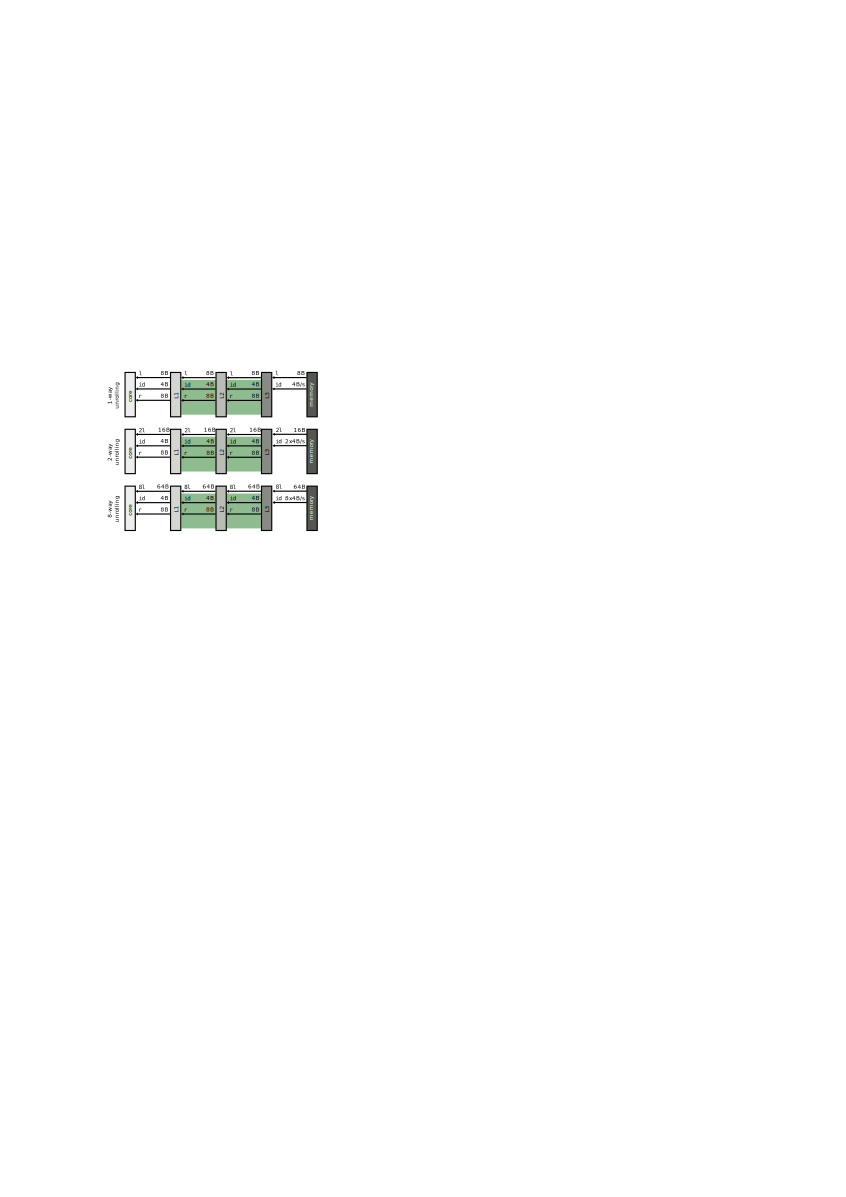
\includegraphics[width=0.75\linewidth,clip=true]{images/ecm-datatransfers-bw}
  \caption{Data transfers for one iteration of the backward
    substitution when $1$-, $2$-, or $8$-way column unrolling is applied
    for a panel with panel size $s$.
    Thereby $1$, $2$, or $8$ nonzero elements of \vlnz{} are processed,
    respectively.
%    Loading of \vindx{} from memory (blue boxes) is only included in the model
%    if the panel size $s \le 8$.
% From which cache level \vr{} is reused (green boxes) depends on the size of the
% active part. If the active part is large it must be reloaded from
% L3 cache. With decreasing size it can fit into L2 or even L1 cache.
% This holds also true for \vindx{}, but additionally depends on the panel size.
  }
  \label{fig:ecm:data-bw}
\end{figure}

\subsection{Data transfers and FLOPs with unrolling}
\label{sec:pm:dt:wu}

%
As noted in Section~\ref{sec:algo} it is beneficial to handle several columns
at once.
%\sout{In PARDISO loops over columns \uwave{are additionally to no unrolling manually $2$- and $8$-times unrolled and used when a panel contains more than one column.}}
For this purpose PARDISO has additionally 2- and 8-way manually unrolled
loops over columns.  These are used when a panel contains more than one column.
With an unrolling factor of two the innermost loop for forward substitution becomes
%
\begin{algorithmic}[1]
  \State nj = nonzero column length
  \For{k = \nxlnz[j] + offset; k < \nxlnz[j+1]; \textcolor{blue}{k += 2}}
      \State row = \nindx[i++]
      \State \nr[row] = \nr[row] - \nr[j] \nlnz[k] \textcolor{blue}{- \nr[j+1] \nlnz[k+nj]}
  \EndFor
\end{algorithmic}%
%\vspace{-\baselineskip}
\noindent%
%
%\sout{\uwave{In contrast to no unrolling per iteration two nonzeros are processed.}}
Instead of processing only one nonzero the 2-way unrolling handles two
nonzeros per iteration.
Hence, four FLOPs are performed and two entries of \vlnz{} are loaded.
Hereby the corresponding element of \vr{} only needs to be loaded once instead of
twice, when processing two elements of \vlnz{}.
All other transfers stay unchanged.
%
In general with a $u$-way unrolling during each iteration, $2 \times u$\,FLOPs
are executed and $u \times 8\,\text{B} + 20\,\text{B}$ are transferred.

Unrolling of the backward substitution loop results in the following code for a
$2$-way unrolling:
%mw2018-06-07: \mycomment{ML: Bin fuer konsistenz: two-way und two-time
%mw2018-06-07: unrolling oder 2-way und 2-time unrolling. MW: OK}
%
\begin{algorithmic}[1]
  \State nj = nonzero column length
  \For{k = \nxlnz[j] + offset; k < \nxlnz[j+1]; \textcolor{blue}{k += 2}}
      \State row = \nindx[i++]
      \State \nr[j]   = \nr[j] - \nlnz[k] \nr[row]
      \State \textcolor{blue}{\nr[j+1]   = \nr[j+1] - \nlnz[k+nj] \nr[row]}
  \EndFor
\end{algorithmic}%
%\vspace{-\baselineskip}
\noindent%
%
Also here four FLOPs per iteration are performed, two entries of \vlnz{} are
loaded and the corresponding element of \vr{} is loaded only once.
%
For a $u$-way unrolling, $2 \times u$\,FLOPs and $u \times 12\,\text{B} +
8\,\text{B}$ are loaded.

As already noted, we assume \vr{} and a panel's current row indices from
\vindx{} are at least cached in LLC or higher cache levels.
%
Unrolling, hereby, only saves transfers inside the cache hierarchy.
The bytes transferred between memory and LLC are left unaffected and depend only
on the panel size.
With larger panel sizes in total, fewer
row indices \vindx{} are needed for the
whole matrix.

\section[Application of modified Berkeley roofline model]{Application of modified Berkeley roofline model on sparse triangular solve}
\label{sec:mrm}

% \begin{table}[tp]
%   \small
%   \centering
%   \begin{tabular}{llcRRRccRRR}
%   \hline
%   \multirow{2}{*}{u}&& \multicolumn{4}{c}{forward}  && \multicolumn{4}{c}{backward} \\
%   \cline{3-6} \cline{8-11}
%    && \mcco{L1} & \mcco{L2} & \mcco{L3} & \mcco{mem} && \mcco{L1} & \mcco{L2} & \mcco{L3} & \mcco{mem}\\
%   \hline
%   1 && 14   & 4 - 14  &  4 - 14  & 4 - 6    && 10   & 4 -  10 & 4 -  10 & 4  - 6 \\ 
%   2 &&  9   & 4 -  9  &  4 -  9  & 4 - 5    &&  7   & 4 -   7 & 4 -   7 & 4  - 5 \\
%   8 && 5.25 & 4 - 5.25&  4 - 5.25& 4 - 4.25 && 4.75 & 4 -  4.75&4 - 4.75& 4  - 4.25 \\
%   \hline
%   \end{tabular}
%   \caption{Code balance $B_c$ [B/F] of forward/backward substitution for
% different unrollings (u) when
% data is fetched from the corresponding level inside the memory hierarchy. Values
% depend on actual panel size $s$ and possible cache reuse.}
%   \label{tab:mrm:bc}
% \end{table}

%xx \begin{table*}[!t]
%xx   \caption{Details of Evaluated Hardware Systems.
%xx % ISA Lists the Latest Extension Supported by the Processor. 
%xx % Read Memory Bandwidth, Floating Point Instructions per Cycle (ADD+MULL and
%xx % FMA Instructions), and Machine Balance is Reported for Scalar Execution.
%xx KNL's Bandwidth Numbers are for DDR Memory.}
%xx % ECM: 2 cy L1/L2 bei HSW/BDW entgegen der Doku 
%xx % STREAM:
%xx % read = summation
%xx % KNL: no-nt, prefetch not explicitly disabled
%xx % ZEN: no-nt, AVX2, only even cores
%xx % HSW2: no-nt, avx2
%xx % HSW: no-nt, avx2
%xx % IVB: no-nt, 
%xx   \label{tab:hw}
%xx   \footnotesize
%xx  \centering
%xx %\resizebox{\textwidth}{!}{%
%xx  \begin{tabular}{p{1.9cm}llrrrrrrrrr}
%xx     \hline
%xx     name      & &  & IVB         & HSW-D      & HSW-S           & BDW           & SKX         & KNL           & ZEN-D        &  ZEN-S         \\
%xx     \hline                                                      
%xx     \multirow{3}{\linewidth}{processor name} & &  & Intel& Intel & Intel & Intel & Intel & Intel & AMD &  AMD \\
%xx       & &  & Xeon  & Xeon & Xeon      & Xeon    & Xeon  & Xeon    &
%xx ~~Ryzen 7   &  ~~EPYC      \\
%xx               & &  &\scriptsize  E5-2660 v2 &\scriptsize  E3-1240 v3
%xx &\scriptsize  E5-2695 v3      &\scriptsize  E5-2630 v4    &\scriptsize  Gold
%xx 6148   &\scriptsize  Phi 7210      &\scriptsize  1700X      &\scriptsize
%xx 745           \\
%xx %     processor & &  & Intel Xeon  & Intel Xeon & Intel Xeon      & Intel Xeon    & Intel Xeon  & Intel Xeon    & AMD Ryzen    &  AMD EPYC      \\
%xx %     name      & &  &  E5-2660 v2 & E3-1240 v3 & E5-2695 v3      & E5-2630 v4    & Gold 6148   & Phi 7210      & 7 1700X      &  745           \\
%xx     \hline                                                      
%xx     micro     & &  & Ivy Bridge  & Haswell    & Haswell         & Broadwell
%xx & Skylake     & ~Knigths       & Zen          &  Zen           \\
%xx     arch.     & &  &             &            &                 &               &             & Landing       & \\
%xx     \hline                                                    
%xx     freq    & [GHz] & & 2.2      & 3.4        & 2.3             & 2.2           & 2.4         & $\approx$ 1.3 & 3.4          &  2.3           \\
%xx     cores   &       & & 10       & 4          & 2 $\times$ 7    & 10            & 20          & 64            &   8          &  24            \\
%xx     ISA     &       & & AVX      & AVX2       & AVX2            & AVX2          & AVX-512     & AVX-512       & AVX2         &  AVX2          \\
%xx %    sockets &       & 2        & 1          & 2               & 2             & 2           & 1             & 1            &  & 1 \\
%xx %    \mltwo{NUMA LDs}& 2        & 1          & 2 $\times$ 2    & 2 $\times$ 2  & 2           & 1             & 1            &  & 1 \\
%xx     \mltwo{NUMA LDs} & & 1       & 1          & 2               & 1             & 1           & 1             & 1            & 4              \\
%xx     \hline                                                    
%xx     L1 & [KiB]     &  &  32      & 32         & 32              & 32            & 32          & 32            & 32           &  32            \\
%xx     L2 & [KiB]     &  &  256     & 256        & 256             & 256           & 1024        & 1024          & 512          &  512           \\
%xx     L3 & [MiB]     &  &  25      & 8          & 2 $\times$ 17.5 & 25            & 28          & -             & 2 $\times$ 8 &  8 $\times$ 8 \\ 
%xx     \hline
%xx %    copy bw. & [GB/s] & 41.2   & 26.6            & 22.6       & 31.3 & ?? &  75.9 & 30.2 & 212 \\ % complete socket/cod
%xx %    read bw. & [GB/s] & 44.3   & 30.9            & 23.6       & 33.7 & ?? &  74.2 & 32.5 & 231 \\ % complete socket/cod
%xx     \mlfour{scalar read bw.}   &     &          &  \\
%xx     ~1 core  & [GB/s]  &&  9.5 & 16.6 & 12.1 & 11.5 &  14.5 &  8.5 & 19.3 & 19.3  \\
%xx     ~NUMA LD & [GB/s]  && 44.4 & 22.7 & 31.2 & 56.3 & 108.0 & 75.2 & 33.7 & 37.6  \\
%xx     \hline
%xx     \mlfour{scalar ADD+MUL/FMA} &&& \\
%xx     ~1 core  & [F/cy] &&  2 &  4 &  4 &  4 &  4 &   4 &  4 &  4 \\
%xx     ~NUMA LD & [F/cy] && 20 & 16 & 28 & 40 & 80 & 256 & 32 & 24 \\
%xx     \hline
%xx     \mlfour{scalar machine balance $B_m$} &  &         & \\
%xx     ~1 core  & [B/F] && 2.2 & 1.2 & 1.3 & 1.3 & 1.5 & 1.6 & 1.4 & 2.1 \\
%xx     ~NUMA LD & [B/F] && 1.0 & 0.4 & 0.5 & 0.6 & 0.6 & 0.2 & 0.3 & 0.7 \\
%xx     \hline
%xx \\[0.01em]
%xx   \end{tabular}
%xx %} % from https://tex.stackexchange.com/a/27105
%xx \end{table*}
%\parbox{.25\linewidth}{ 
%\begin{SCtable}[][t]

For our performance predictions of the sparse triangular solve, we apply the roofline model~(\cite{williams-2009}).
As mentioned before, the model takes into account the attainable memory bandwidth as well as
the
peak floating
point performance of the processor and 
%\uwave{%\sout{correlates}
relates these hardware capabilities %\sout{with}
to
the requirements of the code.
%}
%mw2018-06-07: \mycomment{OR: was heisst dieses? MW: besser? OR: Etwas. Aber inwiefern wird
%mw2018-06-07: eine Beziehung zu den Anforderungen hergestellt? MW: Die Code-Balance $B_c$ ist
%mw2018-06-07: die Anforderung des Codes und $B$ bzw.\ $P_\text{max}$ stammt von der Hardware.}
It can be written as
%
\be
  P = \min(P_\text{max}, B / B_c),
\ee
where $P_\text{max}$ denotes the attainable floating point performance, $B$ the
attainable memory bandwidth, and $B_c$ the code balance.

Here, $P_\text{max}$
depends already on the floating point characteristics of the code and the
processor and does not represent the peak floating point performance as it can
be obtained from a processor's data sheet. 
If a processor supports vectorized FMA instructions, but
only vectorized add or multiply instructions are used, then $P_\text{max}$ is
halved.
Using scalar instructions instead of the AVX vectorized counterparts reduces
$P_\text{max}$ further by a factor of four.
%
And, finally, if the floating point instruction mix does not equally utilize a
processors floating point units, $P_\text{max}$ is again reduced.
% \todo{This is a forward reference.}
For example, the Ivy Bridge (IVB) system (Section~\ref{sec:tb}, Table~\ref{tab:hw}) hosts an add and
multiply unit, but if only one type of floating point instruction is used, only
half of the theoretical floating
point performance can be attained. 
%
In our case the compiler uses 
scalar FMA instructions
for the core loops of the %\sout{forward/backward substitution} 
sparse triangular solve
for architectures
with AVX2 support and scalar \linebreak add/multiply instructions for
architectures without FMA support like IVB.

The attainable memory bandwidth $B$ is measured with a microbenchmark,
ideally resembling the application's memory access pattern. 
For the
sparse triangular solve,
%\sout{\OR the forward/backward substitution}
we use a read-only benchmark from the LIKWID tool suite (\cite{likwid-2010-arxiv}).
%
As the sparse triangular solve
%\sout{\OR the forward/backward substitution}
in PARDISO only uses scalar load instructions we also use them
for the microbenchmark. 

The \textit{code balance} $B_c$ is the ratio of bytes transferred to the
number of FLOPs performed in the code.
In the best case, when the panel size $\panelsize$ is large and the indices are
cached, during the forward~\eqref{eq:algo:fw:pardiso} and backward
substitutions~\eqref{eq:algo:bw:pardiso}, each nonzero of $L$ must be loaded once
and the loading of indices can be neglected,
respectively. 
Furthermore, the computation involves two FLOPs per nonzero.
As nonzeros are stored in double precision consuming $8$\,B, this results in a
best case code balance of $B_c = 8 / 2 \text{B/F} = 4 \text{B/F}$, where F
denotes FLOP.
%1 Table~\ref{tab:mrm:bc} lists the code balance for different unrollings and cache
%1 levels and uses the data transfer and FLOP counts from Sect.~\ref{sec:sds}.
Table~\ref{tab:mrm:bc} lists the code balance for different unrolling factors
when the factor $L$ must be fetched from memory and uses the data transfer and
FLOP counts from Section~\ref{sec:sds}.
In contrast, the \textit{machine balance} $B_m$ defines the ratio for the whole system
and uses the ratio of the attainable memory bandwidth $B$ to the maximum floating point
performance $P_\text{max}$.
% \todo{This is a forward reference.}
% \mycomment{OR: Tab. ist keine erlaubte Abkuerzung f\"ur Table. MW: stimmt}
This bandwidth is found in Table~\ref{tab:hw} for all systems.
%
If $B_c > B_m$ then the roofline model indicates 
that the code's performance is
limited by the memory bandwidth,
i.e., that the code is memory bound.
%1 This is the case for sparse direct solve for all unrollings, when data is
%1 located in L2, L3, or memory.
{This is the case for the sparse %\sout{direct} 
triangular solve 
phase %\sout{for} 
of all
%mw2018-06-07: \uwave{
unrolling factors,
%mw2018-06-07: }
when the factor $L$ is too large to be kept in cache and
completely located in memory.}
%mw2018-06-07: \mycomment{\OR was meint ``unrolling factor'' hier? \MW MW: Das ist der Faktor
%mw2018-06-07: für das ``loop unrolling''. Der Begriff wird vorher auch schon so verwendet,
%mw2018-06-07: daher haette ich den nicht nocheinmal erlaeutert.}

\begin{table}[t]
  \centering
   \begin{tabular}{ll|cm{0.8eM}cm{0.8eM}c|cm{0.8eM}cm{0.8eM}c}
  \hline
  Substitution && \multicolumn{5}{c|}{Forward} & \multicolumn{5}{c}{Backward} \\
  %\cline{3-5} \cline{7-9}
  \hline
     $u$    &     &  1   &  & 2    &  & 8        & 1     &  & 2   &  & 8  \\
     $B_c$  & [B/F]\, & \ $4-6$ & & $4-5$ & & $4-4.25$ \ & \ $4-6$ & & $4-5$ & & $4-4.25$ \ \\
  \hline
  \end{tabular}
  \caption{Code balance $B_c$ of forward/backward substitution for
unrolling factors $u$ when
the factor $L$ must be fetched from memory.
% the factor $L$ exceeds the LLC and must be fetched from memory.
Values depend on actual panel size $s$ and possible cache reuse.}
  \label{tab:mrm:bc}
\end{table}

To determine performance limits, we only consider the case when data reside in
memory.
Therefore the data transfers between the L3 cache and memory are relevant as shown
in Figures~\ref{fig:ecm:data-fw} and \ref{fig:ecm:data-bw}.
Only nonzero entries of $L$ with the corresponding panel indices are loaded. 
Their amount depends only on the structure of $L$ and is independent of the used
loop unrollings.
%
The roofline model for the memory bound case as a function of the number of
threads~$t$ can be formulated as
%
\be
  \label{eq:rm:simple}
  P^{A}(t)
  = \frac{
      \text{nnz} (L) \times 2 \frac { \text{FLOP}}{ \text{nz}}
    }{
     \frac{D_A(t)}{ B(t)} 
    } \quad \frac{\text{FLOP}}{s},
\ee
%
%\mycomment{OR: Genaugenommen sind Einheiten in eckigen Klammern veraltet;
%https://de.wikipedia.org/wiki/Einheitenzeichen MW: OK, die Einheiten in Klammern
%in den Tabellen sollten aber passen.
%OR: Es ist mir nicht so wichtig, es kann auch in eckige Klammern.
%}
where $\text{nnz}(L)$ denotes the number of nonzeros of the factor $L$ 
resulting from a factorization of $A$ for $t$ threads, 
$B(t)$ is the attainable memory bandwidth of the system utilizing $t$ threads, and 
$D_A(t)$ the data volume of nonzeros and indices making up $L$.
The only adjustment to the original model here is its dependency on the number
of threads. 
Choosing $t$ equal to the number of total cores yields the original roofline model.

To distinguish between the parallel phase, where the parts are handled,
and the serial part, where the separator is treated, we modify 
\eqref{eq:rm:simple}.
We use the following formula for the \textit{modified roofline model}: 
%
\be
  \label{eq:rm:mod}
  P^{A}_{\text{mod}}(t) 
  = \frac{
      \text{nnz} (L) \times 2 \frac { \text{FLOP}}{ \text{nz}}
    }{
     \frac{D_A^p(t) }{  B(t) } + \frac{ D_A^s(t) }{ B(1) }
    } \quad \frac{\text{FLOP}}{s},
\ee
%
where
$D_A^p(t)$ 
represents
the data volume of nonzeros and indices %\sout{\uwave{made up}} 
built up
% \mycomment{OR: ``made up''? Erfunden? MW: OK}
by the parallel parts, and $D_A^s(t)$ the data volume %\sout{\uwave{made up}}
built up by the nonzeros and
indices of the separator.
%
Please note that both data volumes $D_A^p(t)$ and $D_A^s(t)$ depend on
$A$ and the number of threads $t$.
%
The values for $D_A^p(t)$ and $D_A^s(t)$ are extracted from the factorized
matrices a priori to solve.

Please note that the accuracy of the roofline model predictions, especially for
single cores, as included in the modified model, can be inaccurate. 
%\mycomment{OR: Auf welches Ganzes bezieht sich ``part''? MW: Done.}
If the in-core execution time (excluding floating point operations) or the in-cache
traffic dominates the execution time, predictions become unreliable as this is not
covered by the roofline model.
In Chapter~\ref{sec:performance}, we use dedicated single core measurements to
validate that, in the case of the sparse triangular solve,
%\sout{\OR the forward/backward substitution,}
this approach is valid. 
%
However, this effect can be modeled in detail with the ECM
model (\cite{treibig-2010-ecm, hager-2012-ecm, stengel-2015}) and was already
studied for stencil kernels.


%-- \begin{table*}[!t]
%-- \parbox{.7\linewidth}{
%--   \caption{Details of Evaluated Hardware Systems.
%-- % ISA Lists the Latest Extension Supported by the Processor. 
%-- % Read Memory Bandwidth, Floating Point Instructions per Cycle (ADD+MULL and
%-- % FMA Instructions), and Machine Balance is Reported for Scalar Execution.
%-- KNL's Bandwidth Numbers are for DDR Memory.}
%-- % ECM: 2 cy L1/L2 bei HSW/BDW entgegen der Doku 
%-- % STREAM:
%-- % read = summation
%-- % KNL: no-nt, prefetch not explicitly disabled
%-- % ZEN: no-nt, AVX2, only even cores
%-- % HSW2: no-nt, avx2
%-- % HSW: no-nt, avx2
%-- % IVB: no-nt, 
%--   \label{tab:hw}
%--   \footnotesize
%--  \centering
%-- %\resizebox{\textwidth}{!}{%
%--  \begin{tabular}{p{1.9cm}llrrrrrrrrr}
%--     \hline
%--     name      & &  & IVB         & HSW-D      & HSW-S           & BDW           & SKX         & KNL           & ZEN-D        &  ZEN-S         \\
%--     \hline                                                      
%--     \multirow{3}{\linewidth}{processor name} & &  & Intel& Intel & Intel & Intel & Intel & Intel & AMD &  AMD \\
%--       & &  & Xeon  & Xeon & Xeon      & Xeon    & Xeon  & Xeon    &
%-- ~~Ryzen 7   &  ~~EPYC      \\
%--               & &  &\scriptsize  E5-2660 v2 &\scriptsize  E3-1240 v3
%-- &\scriptsize  E5-2695 v3      &\scriptsize  E5-2630 v4    &\scriptsize  Gold
%-- 6148   &\scriptsize  Phi 7210      &\scriptsize  1700X      &\scriptsize
%-- 745           \\
%-- %     processor & &  & Intel Xeon  & Intel Xeon & Intel Xeon      & Intel Xeon    & Intel Xeon  & Intel Xeon    & AMD Ryzen    &  AMD EPYC      \\
%-- %     name      & &  &  E5-2660 v2 & E3-1240 v3 & E5-2695 v3      & E5-2630 v4    & Gold 6148   & Phi 7210      & 7 1700X      &  745           \\
%--     \hline                                                      
%--     micro     & &  & Ivy Bridge  & Haswell    & Haswell         & Broadwell
%-- & Skylake     & ~Knigths       & Zen          &  Zen           \\
%--     arch.     & &  &             &            &                 &               &             & Landing       & \\
%--     \hline                                                    
%--     freq    & [GHz] & & 2.2      & 3.4        & 2.3             & 2.2           & 2.4         & $\approx$ 1.3 & 3.4          &  2.3           \\
%--     cores   &       & & 10       & 4          & 2 $\times$ 7    & 10            & 20          & 64            &   8          &  24            \\
%--     ISA     &       & & AVX      & AVX2       & AVX2            & AVX2          & AVX-512     & AVX-512       & AVX2         &  AVX2          \\
%-- %    sockets &       & 2        & 1          & 2               & 2             & 2           & 1             & 1            &  & 1 \\
%-- %    \mltwo{NUMA LDs}& 2        & 1          & 2 $\times$ 2    & 2 $\times$ 2  & 2           & 1             & 1            &  & 1 \\
%--     \mltwo{NUMA LDs} & & 1       & 1          & 2               & 1             & 1           & 1             & 1            & 4              \\
%--     \hline                                                    
%--     L1 & [KiB]     &  &  32      & 32         & 32              & 32            & 32          & 32            & 32           &  32            \\
%--     L2 & [KiB]     &  &  256     & 256        & 256             & 256           & 1024        & 1024          & 512          &  512           \\
%--     L3 & [MiB]     &  &  25      & 8          & 2 $\times$ 17.5 & 25            & 28          & -             & 2 $\times$ 8 &  8 $\times$ 8 \\ 
%--     \hline
%-- %    copy bw. & [GB/s] & 41.2   & 26.6            & 22.6       & 31.3 & ?? &  75.9 & 30.2 & 212 \\ % complete socket/cod
%-- %    read bw. & [GB/s] & 44.3   & 30.9            & 23.6       & 33.7 & ?? &  74.2 & 32.5 & 231 \\ % complete socket/cod
%--     \mlfour{scalar read bw.}   &     &          &  \\
%--     ~1 core  & [GB/s]  &&  9.5 & 16.6 & 12.1 & 11.5 &  14.5 &  8.5 & 19.3 & 19.3  \\
%--     ~NUMA LD & [GB/s]  && 44.4 & 22.7 & 31.2 & 56.3 & 108.0 & 75.2 & 33.7 & 37.6  \\
%--     \hline
%--     \mlfour{scalar ADD+MUL/FMA} &&& \\
%--     ~1 core  & [F/cy] &&  2 &  4 &  4 &  4 &  4 &   4 &  4 &  4 \\
%--     ~NUMA LD & [F/cy] && 20 & 16 & 28 & 40 & 80 & 256 & 32 & 24 \\
%--     \hline
%--     \mlfour{scalar machine balance $B_m$} &  &         & \\
%--     ~1 core  & [B/F] && 2.2 & 1.2 & 1.3 & 1.3 & 1.5 & 1.6 & 1.4 & 2.1 \\
%--     ~NUMA LD & [B/F] && 1.0 & 0.4 & 0.5 & 0.6 & 0.6 & 0.2 & 0.3 & 0.7 \\
%--     \hline
%-- \\[0.01em]
%--   \end{tabular}
%-- %} % from https://tex.stackexchange.com/a/27105
%-- }
%-- %\end{table*}
%-- \parbox{.25\linewidth}{ 
%-- %\begin{SCtable}[][t]
%-- %\begin{table}[tp]
%--   \caption{Dimension ($n$) and number of nonzeros ($\text{nnz}$) for $A$ and 
%-- $L$ for all benchmark matrices.}
%--   \label{tab:m:list}
%--   \centering
%--   \small
%--   \begin{tabular}{ll|rrrrrr}
%--   \hline
%--   matrix      &&  \multicolumn{1}{c}{${n}$} &&
%--             \multicolumn{1}{c}{${\text{nnz}(A)}$}  &&
%--             \multicolumn{1}{c}{${\text{nnz}(L)}$}   \\ 
%-- %  {\bfseries matrix}      &&  \multicolumn{1}{c}{$\bm{n}$} &&
%-- %            \multicolumn{1}{c}{$\bm{\text{nnz}(A)}$}  &&
%-- %            \multicolumn{1}{c}{$\bm{\text{nnz}(L)}$}   \\ 
%--   \hline
%-- % values for threads = 1, p = 80
%--   dense  && $    20 \times 10^3$ && $200 \times 10^6$ &&  $  200 \times 10^6$  \\ % ps-n-20000-t-1-p-80
%--   lapl1  && $   256 \times 10^3$ && $  3 \times 10^6$ &&  $  219 \times 10^6$  \\ % pl-n-40-b-4-t-1-p-80  N=40, B=4
%--   lapl2  && $   343 \times 10^3$ && $  1 \times 10^6$ &&  $  166 \times 10^6$  \\ % pl-n-70-b-1-t-1-p-80  N=70, B=1
%--   omen1  && $1\,751 \times 10^3$ && $ 32 \times 10^6$ && $1\,076 \times 10^6$  \\ % omen-rc2.5-lc160-t-1-p-80
%--   omen2  && $   760 \times 10^3$ && $ 20 \times 10^6$ && $   690 \times 10^6$  \\ % omen-rc3.5-t-1-p-80
%--   omen3  && $1\,271 \times 10^3$ && $ 42 \times 10^6$ && $1\,651 \times 10^6$  \\ % omen-rc4.5-t-1-p-80
%--   bddc   && $   750 \times 10^3$ && $ 31 \times 10^6$ && $1\,590 \times 10^6$  \\ % mat\_Kii\_sd22\_size750141\_load2\_newton1
%--   \hline
%--   \end{tabular}
%-- }\vfill{}
%-- %\end{table}
%-- %\end{SCtable}
%-- \end{table*}

\section{Application of Erlangen ECM model on sparse triangular solve}
\label{sec:ecm-fwbw}

As shown in Chapter \ref{sec:sds}, there are many factors influencing the performance. For example unrolling, active part of \vr{} or if \vindx{} is already loaded in cache or not. Detailed performance evaluation would require a model for every combination of these parameters and combining these models based on detailed analysis of a matrix $A$ and its factor $L$. For real world matrices, this is not possible.
To make the modeling feasible, we focus only on two extreme cases: first, we consider the code without unrolling that reads \vindx{} from the memory and second, 8-way unrolled code that already has \vindx{} in cache. In both cases we are assuming the active part of \vr{} is large and the data reside in the L3 cache. The first scenario achieves the worst possible performance, while the second one can perform close to the theoretical maximum. These two cases give us a range of expected performance, such that for any matrix the sparse triangular solve algorithm should be within these bounds.

%\todop{Worst case}
%Processing one element of \vlnz{} without unrolling takes 2 FLOPs and requires 28\,B or 20\,B transfered between cache levels or registers for forward and backward substitution, respectively, and 12\,B are read from memory.
For the ECM model of the worst case we consider eight iterations of the inner most loop (8 rows) in order to fill one cache line.
Eight iterations of both forward and backward substitution without unrolling require sixteen $8$\,B loads (\verb|r[:]| and \verb|l[:]|) and eight $4$\,B loads (\verb'idx[:]').
On top of that, the forward substitution also requires eight $8$\,B stores (\verb'r[:]').
These loads and stores need $32$ addresses (forward substitution) or $24$ addresses (backward substitution) to be generated, which takes $16$ or $12$ cycles, respectively. We assume that all the addresses are generated on ports 2 and 3. The simple AGU on port 7 is not used as we showed in Sections~\ref{sec:epm} and \ref{sec:ecm-indirect-daxpy}.
The floating point arithmetics for eight iterations consists of 8 multiplications and 8 additions. This can be done in 8 cycles using the units on ports 0 and 1.
Unlike in the DAXPY case, only 96\,B (or 1.5\,cl) are read from memory.
This leads to expected performance of 1.18\,GF/s (forward substitution) or 1.46\,GF/s (backward substitution).

%\todop{Best case}
For the ECM model of the best case with 8-way unrolling we take 8 columns and in every column 8 rows (8 iterations of the innermost loop).
Eight iterations of forward substitution with 8-way unrolling require 672\,B (10.5\,cl) to be loaded from cache and 512\,B (8\,cl) read from memory.
Backward substitution require 608\,B (9.5\,cl) to be loaded from cache and 512\,B (8\,cl) read from memory.
These loads and stores need $88$ addresses (forward substitution) or $80$ addresses (backward substitution) to be generated, which takes $44$ or $40$ cycles, respectively.
The floating point arithmetics consist of 64 multiplications and 64 additions. This can be done in 64 cycles.
In the best case we assume \vindx{} is kept in the cache, thus only 512\,B (8\,cl) are read from memory.
This leads to expected performance 2.7\,GF/s (forward substitution) or 2.86\,GF/s (backward substitution).

\todol{ref images}


\begin{comment}
%For the ECM model we consider 8 sequential iterations of the innermost loop, which fill one 64\,B cache line.

\todop{ \\
Algorithm similar to indexed daxpy (Section \ref{sec:ecm-indirect-daxpy}). \\
Detailed description of the algorithm in Chapter \ref{sec:algo}. \\
Analysis of the code including unrolling in Chapter \ref{sec:sds}. \\
\\
Computations here\\
Elements form L are used only once, hence they are always fetched from the memory. We can ignore the tL1..tL3. \\
\\}

In this section we describe ECM model of the forward forward (Algorithm~\ref{alg:algo:fw}) and backward (Algorithm~\ref{alg:algo:bw}) substitution. We focus our attention on the inner-most loop iterating over rows with nonzero entries in a column.

The forward substitution is an indexed DAXPY kernel analyzed in Section~\ref{sec:ecm-indirect-daxpy}, but for the forward substitution we have different assumptions regarding where the data reside. Moreover the code is unrolled, processing several columns at once, which reduces the data transfers.
\todol{continue here}
The overlapping part of in-core execution is exactly the same as in the indirect daxpy.
Again we take 8 iterations (or 8 rows) as an unit of work, because it fills one cache line. Note that the supernodes in L are stored column-wise, ignoring the sparsity, as described in Chapter \ref{sec:algo}.
We will take into account 1 column for 1-way unroling, 2 columns for 2-way unrolling and 8 columns for 8-way unrolling.
This gives
\begin{eqnarray}
   t^1_\text{ol} & = & \ \ 6\,\cyw \\
   t^2_\text{ol} & = & 12\,\cyw \\
   t^8_\text{ol} & = & 48\,\cyw
\end{eqnarray}

In PARDISO always the most efficient code is used. When a supernode has eight or more columns, the 8-way unrolling is used. 2-way unrolling is used for the remining columns and 1-way unrolling is used only for one column, in case the number of columns is odd.
id is loaded only once per supernode. It could happen in any of the code variants 1-, 2- or 8-way unrolled, depending on the size of the supernode, as shown in Figure \ref{fig:ecm:data}.
We assume id is always loaded from memory in the 1-way unrolled code and for the 2- or 8-way unrolled code it is already present in cache. This allows us to keep the model simple and independent of the nonzero structure of the matrix and its factor L.

In the indexed daxpy r was loaded and stored from/to memory. The right hand side is often assembled just before calling the forward and backward substitution, so it is reasonable to assume that r is already in the cache. We also assume r is small enough to fit the L3 (LLC) cache and as it is used again and again, so it is not evicted.
In case that r was not already present in the cache, it has to be loaded from memory. For reasonably big matrices we can ignore this load from memory, as it happens only once, and assume it is always present in the cache.

There is one difference between the forward and backward substitution in the access pattern to r.
The forward substituion updates different entries in r, the backward substitution always updates the same entry. The updated values in the forward substitution need to be stored in cache after every update (red text and arrows in Figure \ref{fig:ecm:data}), while the only value updated in the backward substituion is kept in register.

Eight iterations of both forward and backward substitution (1-way unrolled) require sixteen $8$\,B loads (\verb|r[:]| and \verb|l[:]|) and eight $4$\,B loads (\verb'idx[:]').
On top of that the forward substitution also requires eight $8$\,B stores (\verb'r[:]').
These loads and stores need $32$ addresses (forward substitution) or $24$ addresses (backward substitution) to be generated, which takes $16$ or $12$ cycles, respectively. We assume all the addresses are generated on ports 2 and 3. The simple AGU on port 7 is not used as we showed in Sections \ref{sec:epm} and \ref{sec:ecm-indirect-daxpy}.
\todol{use 1 row as an unit of work?}

\todop{
ops, cycles, normalized \\
32 24 16 12 16 12 \\
40 32 20 16 10 8 \\
88 80 44 40 5.5 5
}

The floating ponit arithmetics for eight iterations in one column (1-way unrolled) consists of 8 multiplications and 8 additions. This can be done in 8 cycles using the units on ports 0 and 1. The 2- and 8-way unrolled code processes 2 or 8 columns, which require 16 or 64 additions and multiplications respectively. Hence the overlapping part of in-core execution takes 16 cycles for 2-way unrolled code and 64 cycles for 8-way unrolled code.

Unlike in the daxpy case, the amount of data transfered between adjacent cache levels or L1 and registers is different from what is transfered between L3 and memory. We define the work to be for the forward substitution
\begin{eqnarray}
   W^{\text{fw}-1}_\text{cache} & = & 224\,\Bw \\
   W^{\text{fw}-1}_\text{mem}   & = & 96\,\Bw \\
   W^{\text{fw}-2}_\text{cache} & = & 288\,\Bw \\
   W^{\text{fw}-2}_\text{mem}   & = & 128\,\Bw \\
   W^{\text{fw}-8}_\text{cache} & = & 672\,\Bw \\
   W^{\text{fw}-8}_\text{mem}   & = & 512\,\Bw
\end{eqnarray}
and for the backward substitution
\begin{eqnarray}
   W^{\text{bw}-1}_\text{cache} & = & 160\,\Bw \\
   W^{\text{bw}-1}_\text{mem}   & = & 96\,\Bw \\
   W^{\text{bw}-2}_\text{cache} & = & 224\,\Bw \\
   W^{\text{bw}-2}_\text{mem}   & = & 128\,\Bw \\
   W^{\text{bw}-8}_\text{cache} & = & 608\,\Bw \\
   W^{\text{bw}-8}_\text{mem}   & = & 512\,\Bw
\end{eqnarray}
For details please refer to Figure \ref{fig:ecm:data}.

The inputs for the ECM model are summarized in Table \ref{tab:ecm:data}. The values are for clarity normalized for 1 column.

\begin{table}[!t]
  \centering
  \begin{tabular}{|l|c|c|c|c|c|c|c|}
     \hline
     \multicolumn{2}{|c|}{} & \multicolumn{3}{c|}{forward} & \multicolumn{3}{c|}{backward} \\
     \cline{3-8}
     \multicolumn{2}{|c|}{} & 1-way & 2-way & 8-way & 1-way & 2-way & 8-way \\
     \hline
     $W_\text{cache}$ & [B] & 224 & 144 & 84 & 160 & 112 & 76 \\
     $W_\text{mem}$ & [B] & 96 & 64 & 64 & 96 & 64 & 64 \\
     \hline
     tol & [cy] & 8 & 8 & 8 & 8 & 8 & 8 \\
     \hline
     tL1 & [cy] & 16 & 10 & 5.5 & 12 & 8 & 5 \\
     tL2 & [cy] & 3.5 & 2.25 & 1.3125 & 2.5 & 1.75 & 1.1875 \\
     tL3 & [cy] & 3.5 & 2.25 & 1.3125 & 2.5 & 1.75 & 1.1875 \\
     tmem & [cy] & 8.25 & 5.5 & 5.5 & 8.25 & 5.5 & 5.5 \\
     \hline
     Pmem & [GB/s] & 16.5 & 16.6 & 14.2 & 14.6 & 15.2 & 13.6 \\
     Pmem & [GF/s] & 1.18 & 1.84 & 2.7 & 1.46 & 2.16 & 2.86 \\
     \hline
  \end{tabular}
  \caption{\todol{...}}
  \label{tab:ecm:data}
\end{table}
\end{comment}

\section{Experimental testbed for the performance evaluation}
\label{sec:tb}

The specifications of the systems used for the performance analysis are described
in Table~\ref{tab:hw}.
%
The machines with Intel processors are based on the Ivy Bridge (IVB), Haswell
(HSW-D and HSW-S), Broadwell (BDW), Skylake (SKX), and Knights Landing (KNL)
microarchitectures.
The first four microarchitectures are successors to each other and can be seen
as traditional superscalar, multicore, SIMD capable processors.
HSW-D and HSW-S are desktop and server systems, respectively.
The HSW-S systems has cluster-on-die (CoD) enabled.
Here, the processor's local L3 cache is divided into two parts and the memory
forms two NUMA locality domains.
%
SKX is the server variant of the Skylake microarchitecture including support for
AVX-512 and hosts an additional FMA unit.
%
The Knights Landing processor is
%, in contrast to the previously mentioned processors,
a representative of Intels Xeon Phi line, a manycore
architecture with SIMD lanes wider than in the formerly named processors.
It is the successor of the Knights Corner manycore processor.

The exact AVX-512 ISA (instruction set architecture) for Knights Lading differs from the Skylake incarnation,
but for our purpose is not relevant.
Knights Lading includes a $16$\,GB large high bandwidth memory (HBM) with
bandwidths up to $450$\,GB/s; see also the discussion in Chapter~\ref{sec:pa}.
We operate KNL in the flat memory model, where the DDR memory and HBM
represent a NUMA domain, each.
%
AMD-based systems include a desktop (ZEN-D) and server (ZEN-S) system based on the Zen
microarchitecture.
ZEN-S' processor with $24$ cores consists of four NUMA LDs.
%

The CPU frequencies on all machines were fixed to the base frequencies specified
in Table~\ref{tab:hw}.
On the ZEN systems we set the frequency to the nominal base frequency, but could
not disable AMD's turbo mode, which allows cores to run above this frequency.
For Knights Landing, altering frequencies are not supported and are handled by the
processor itself.
%
Furthermore, each thread's affinity was explicitly set.
%
For all arrays, large $2$~MiB pages were used.
%1 This was achieved by using transparent huge pages
%1 \footnote{\texttt{/sys/kernel/mm/transparent\_hugepage/[enabled|defrag]} were set to
%1 \texttt{always}.} as well as calling \texttt{madvise(MADV\_HUGEPAGE)} after
%1 allocation of memory.
%
First-touch policy was in place, and we verified via the NUMA-API that the data
always reside in the cores associated NUMA domain.
%
On all systems supporting simultaneous multithreading (SMT) only physical cores were used.
%
As compiler, Intel C/Fortran Compiler version 17.0.1 was used.

\subsection{Read-only memory bandwidth and machine balance}
\label{sec:tb:membw}

\begin{figure}[!t]%
  \centering%
  \captionsetup[subfigure]{farskip=0pt}%
  \subfloat[]{%
    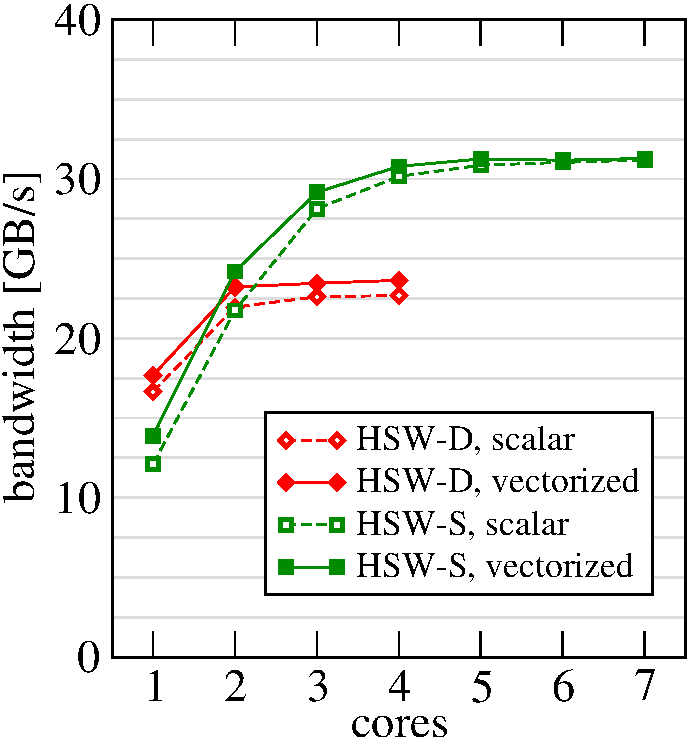
\includegraphics[height=0.4\linewidth,clip=true]{images/stream/StreamReadHswScalarVectorized}
    \label{fig:mrm:bw-scaling}
  } \, \hspace{0.5cm}
  \subfloat[]{%
    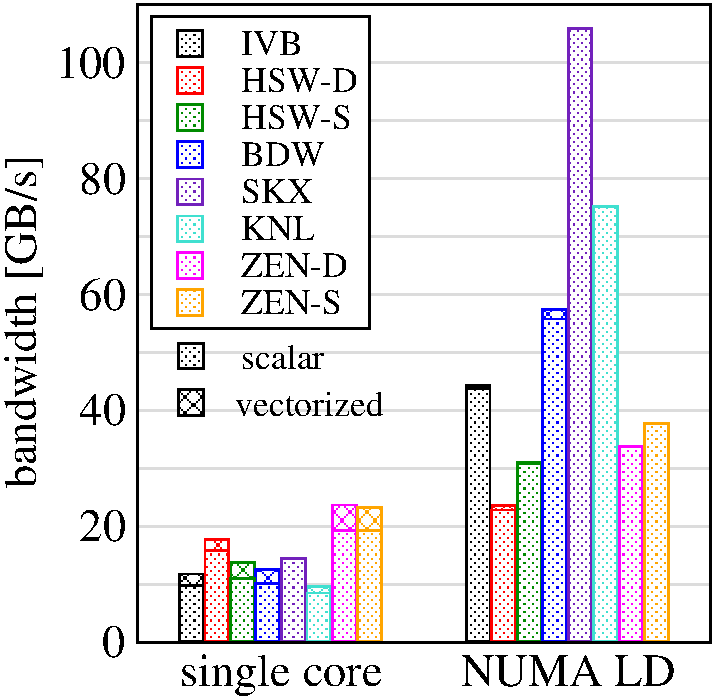
\includegraphics[height=0.4\linewidth,clip=true]{images/stream/StreamReadSingleCoreFullProcessor}
    \label{fig:mrm:bw-single-core}
  }%
  \caption{\protect\subref{fig:mrm:bw-scaling} Bandwidth over the number of cores of the read only benchmark in a
scalar and vectorized version exemplified on HSW-D and
HSW-S.
\protect\linebreak
\protect\subref{fig:mrm:bw-single-core} Single core bandwidth and saturated bandwidth with all available cores of the
processor/cluster.}
  \label{fig:mrm:bw}
\end{figure}

For the performance model an effective memory bandwidth is required.
For the evaluation of the effective bandwidth we measure read-only bandwidth.
The measurements are reported in Table~\ref{tab:hw}.
As discussed in Section~\ref{sec:mrm} only scalar loads are used.
%
If enough cores are used then both scalar and vectorized read-only benchmarks
saturate the memory bandwidth with the only difference being that the saturation of
the latter is already achieved with fewer cores.
This is exemplified on HSW-D and HSW-S systems shown in
Figure~\ref{fig:mrm:bw-scaling}.
HSW-D and HSW-S show the typical saturation behavior for (current Intel) desktop
and server systems.
Typically desktop systems nearly saturate the memory bandwidth with one core.
%
Figure~\ref{fig:mrm:bw-single-core} shows the difference between the scalar and
vectorized read-only benchmark for the single core and the usage of all cores
inside a NUMA LD over all systems in the test bed.
IVB, HSW-S, and the ZEN-based
systems reach,
with one core and vector loads between $15\,\%$ and
$25\,\%$,
a higher bandwidth
than with scalar load instructions.
However, utilizing the full NUMA LD, nearly no difference is visible.
%

% \section{Machine Balance $B_m$}
The machine balance $B_m$ from Table~\ref{tab:hw} considers the scalar read-only
memory bandwidths and the scalar double precision floating point capabilities of
the processors.
This is either a scalar FMA or, if unavailable, a scalar addition and
multiplication for processing a nonzero.

\subsection{Matrices for performance modeling}

\begin{table*}[t]
  \centering
  \small
  \begin{tabular}{ll|rrrrrr}
  \hline
  Matrix      &&  \multicolumn{1}{c}{${n}$} &&
            \multicolumn{1}{c}{${\text{nnz}(A)}$}  &&
            \multicolumn{1}{c}{${\text{nnz}(L)}$}   \\
%  {\bfseries matrix}      &&  \multicolumn{1}{c}{$\bm{n}$} &&
%            \multicolumn{1}{c}{$\bm{\text{nnz}(A)}$}  &&
%            \multicolumn{1}{c}{$\bm{\text{nnz}(L)}$}   \\
  \hline
% values for threads = 1, p = 80
  dense  && $    20 \times 10^3$ && $200 \times 10^6$ &&  $  200 \times 10^6$  \\ % ps-n-20000-t-1-p-80
  lapl1  && $   256 \times 10^3$ && $  3 \times 10^6$ &&  $  219 \times 10^6$  \\ % pl-n-40-b-4-t-1-p-80  N=40, B=4
  lapl2  && $   343 \times 10^3$ && $  1 \times 10^6$ &&  $  166 \times 10^6$  \\ % pl-n-70-b-1-t-1-p-80  N=70, B=1
  omen1  && $1\,751 \times 10^3$ && $ 32 \times 10^6$ && $1\,076 \times 10^6$  \\ % omen-rc2.5-lc160-t-1-p-80
  omen2  && $   760 \times 10^3$ && $ 20 \times 10^6$ && $   690 \times 10^6$  \\ % omen-rc3.5-t-1-p-80
  omen3  && $1\,271 \times 10^3$ && $ 42 \times 10^6$ && $1\,651 \times 10^6$  \\ % omen-rc4.5-t-1-p-80
  bddc   && $   750 \times 10^3$ && $ 31 \times 10^6$ && $1\,590 \times 10^6$  \\ % mat\_Kii\_sd22\_size750141\_load2\_newton1
  \hline
  \end{tabular}
  \caption{Dimension ($n$) and number of nonzeros ($\text{nnz}$) for $A$ and
$L$ for all benchmark matrices.}
  \label{tab:m:list}
%}\vfill{}
%\end{table}
%\end{SCtable}
\end{table*}


Table~\ref{tab:m:list} lists matrix dimension ($n$), number of nonzeros in the
matrix ($\text{nnz}(A)$), and the factor (nnz$(L)$) of the matrices used for
benchmarking in the following sections.
The reported numbers of nonzeros
are reported for factorizations using single threaded execution
and a panel size $\panelsize = 80$.
All matrices are sparse except
for the first matrix \mymat{dense}, where both the matrix and
the factor $L$ are dense.
We use this dense matrix as a best case example for our single core performance
investigations.
The matrices \mymat{lapl1} and \mymat{lapl2} are test matrices arising from a
finite difference discretization of the Laplace operator in three dimensions
with Dirichlet boundary conditions.
In addition, the matrix \mymat{lapl2} contains a block structure
of size $4$.
The \mymat{omen} matrices correspond to a set of representative matrices from
an atomistic nanoelectronic device engineering simulation code (\cite{luisier2011atomistic}).
The matrix \mymat{bddc} arises from a finite element discretization of a typical
solid mechanics problem. Here, as a material model, a J2-elasto-plasticity model
was chosen and three-dimensional and piecewise quadratic tetrahedral finite
elements were used for the discretization. The matrix \mymat{bddc} represents a
typical subdomain problem arising in the BDDC (balancing domain decomposition by
constraints) implicit finite element solver.
Figure \ref{fig:m:spy} shows the structure of A for different matrix classes, whereas more interesting, is the nonzero distribution over the panel sizes of the factor L found in Figure \ref{fig:m:hist}.
Please note that the current factorization limits the number of parts to powers
of two.
To avoid load imbalance during the solve step we report results only for thread
counts which are powers of two.

\begin{figure}[tp]
  \centering
  \captionsetup[subfigure]{farskip=0pt}%
  \subfloat[lapl]{%
    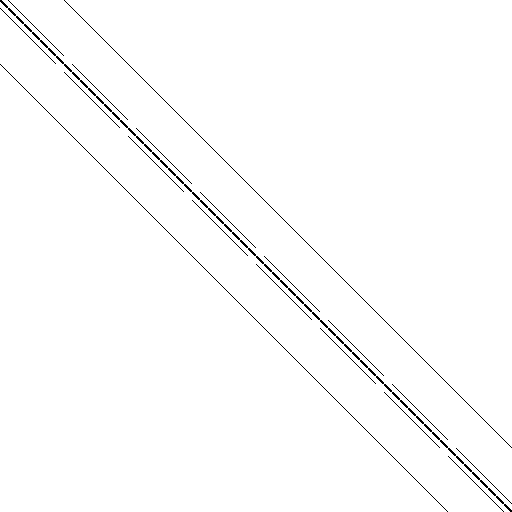
\includegraphics[width=0.25\linewidth,clip=true]{images/spy-plots/a-pl-n-8-b-1}
    \label{fig:m:spy:lp}
  }\,
  \subfloat[omen]{%
    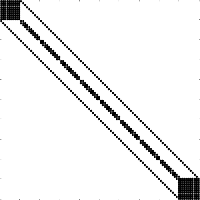
\includegraphics[width=0.25\linewidth,clip=true]{images/spy-plots/omen}
    \label{fig:m:spy:omen}
  }\,
  \subfloat[bddc]{%
    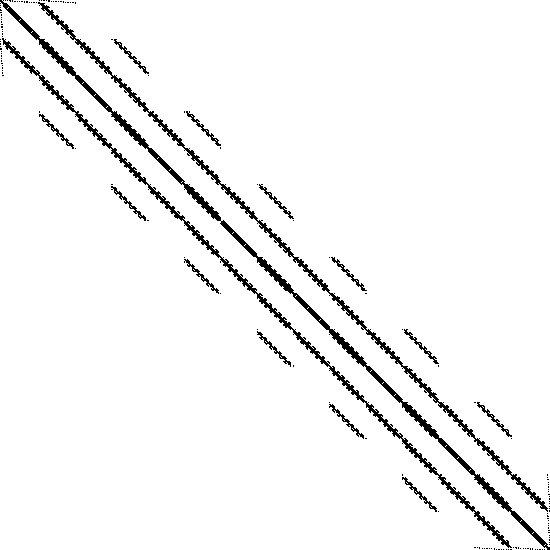
\includegraphics[width=0.25\linewidth,clip=true]{images/spy-plots/mat_Kii_sd89_size10992_load2_newton1}
    \label{fig:m:spy:feti}
  }
  \caption{Structure of $A$ for matrix classes lapl~\protect\subref{fig:m:spy:lp},
  omen~\protect\subref{fig:m:spy:omen}, and bddc~\protect\subref{fig:m:spy:feti}.}
  \label{fig:m:spy}
\end{figure}

\begin{figure*}[tp]
  \centering
  \subfloat[dense]{%
	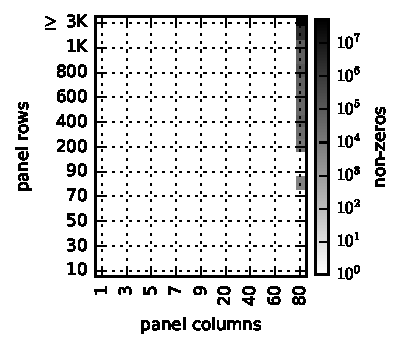
\includegraphics[width=0.3\textwidth,clip=true]{images/matrices/ps-n-20000-t-1-p-80}
	\label{fig:m:hist:dense}
  } \,
  \subfloat[lapl1]{%
	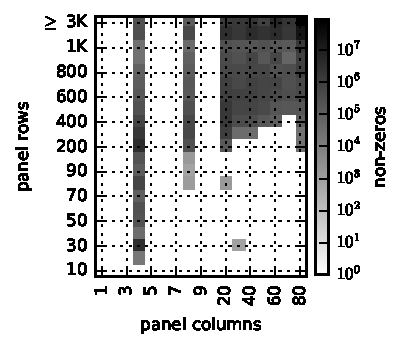
\includegraphics[width=0.3\textwidth,clip=true]{images/matrices/pl-n-00040-b-004}
	\label{fig:m:hist:laplace:n40b4}
  } \,
  \subfloat[lapl2]{%
	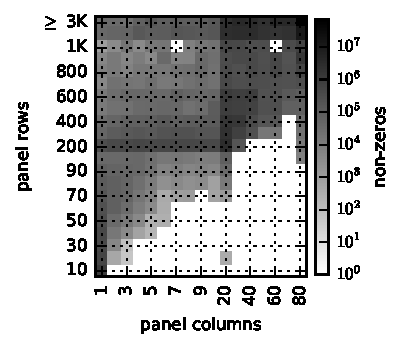
\includegraphics[width=0.3\textwidth,clip=true]{images/matrices/pl-n-70-b-1-t-1-p-80}
	\label{fig:m:hist:laplace:n70b1}
  } \,
  \subfloat[omen1]{%
	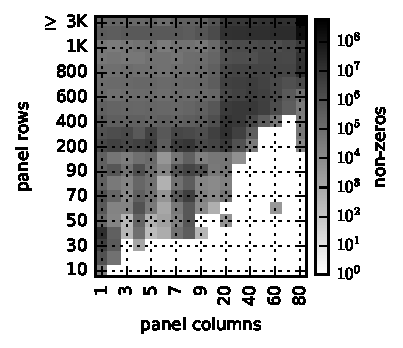
\includegraphics[width=0.3\textwidth,clip=true]{{{images/matrices/omen-rgf-tc2.5-lc160-t-1-p-80.hist-rhs-update-frequencies}}}
	\label{fig:m:hist:omen1}
  } \,
  \subfloat[omen2]{%
	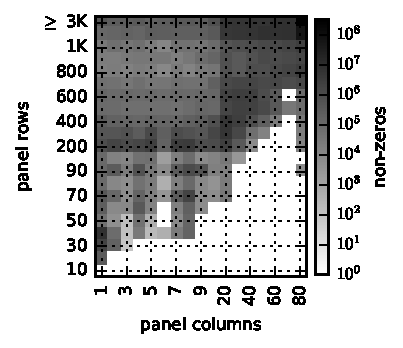
\includegraphics[width=0.3\textwidth,clip=true]{{{images/matrices/omen-rgf-tc3.5-t-1-p-80.hist-rhs-update-frequencies}}}
	\label{fig:m:hist:omen2}
  } \,
%  \subfloat[omen3]{%
%	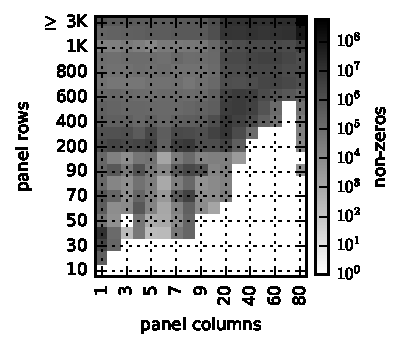
\includegraphics[width=0.3\textwidth,clip=true]{{{images/matrices/omen-rgf-tc4.5-t-1-p-80.hist-rhs-update-frequencies}}}
%	\label{fig:m:omen}
%  } \,
  \subfloat[feti1]{%
	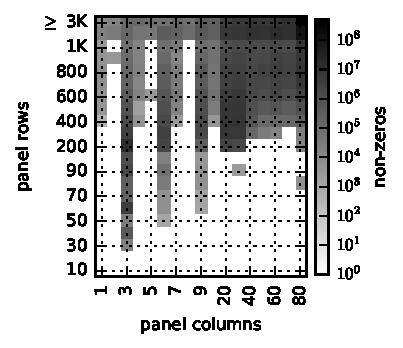
\includegraphics[width=0.3\textwidth,clip=true]{{{images/matrices/mat_Kii_sd22_size750141_load2_newton1-t-1-p-80.log-rhs-update-frequencies}}}
	\label{fig:m:hist:feti1}
  } \,
  \caption{Multiparameter histograms showing how many nonzeros of L are in panels with a certain number of columns and rows. Panels with 3000 and more rows are accumulated. This plot gives an impression of how the work, i.e., nonzeros, in L is distributed over panel dimensions.}
  \label{fig:m:hist}
\end{figure*}
